\documentclass[sigconf]{acmart}

\usepackage{booktabs} % For formal tables


% Copyright
%\setcopyright{none}
%\setcopyright{acmcopyright}
%\setcopyright{acmlicensed}
\setcopyright{rightsretained}
%\setcopyright{usgov}
%\setcopyright{usgovmixed}
%\setcopyright{cagov}
%\setcopyright{cagovmixed}


% DOI
\acmDOI{10.475/123_4}

% ISBN
\acmISBN{123-4567-24-567/08/06}

%Conference
\acmConference[WOODSTOCK'97]{ACM Woodstock conference}{July 1997}{El
  Paso, Texas USA} 
\acmYear{1997}
\copyrightyear{2016}

\acmPrice{15.00}


\begin{document}
\title{SIG Proceedings Paper in LaTeX Format}
\titlenote{Produces the permission block, and
  copyright information}
\subtitle{Extended Abstract}
\subtitlenote{The full version of the author's guide is available as
  \texttt{acmart.pdf} document}


\author{Ben Trovato}
\authornote{Dr.~Trovato insisted his name be first.}
\orcid{1234-5678-9012}
\affiliation{%
  \institution{Institute for Clarity in Documentation}
  \streetaddress{P.O. Box 1212}
  \city{Dublin} 
  \state{Ohio} 
  \postcode{43017-6221}
}
\email{trovato@corporation.com}

\author{G.K.M. Tobin}
\authornote{The secretary disavows any knowledge of this author's actions.}
\affiliation{%
  \institution{Institute for Clarity in Documentation}
  \streetaddress{P.O. Box 1212}
  \city{Dublin} 
  \state{Ohio} 
  \postcode{43017-6221}
}
\email{webmaster@marysville-ohio.com}

\author{Lars Th{\o}rv{\"a}ld}
\authornote{This author is the
  one who did all the really hard work.}
\affiliation{%
  \institution{The Th{\o}rv{\"a}ld Group}
  \streetaddress{1 Th{\o}rv{\"a}ld Circle}
  \city{Hekla} 
  \country{Iceland}}
\email{larst@affiliation.org}

\author{Lawrence P. Leipuner}
\affiliation{
  \institution{Brookhaven Laboratories}
  \streetaddress{P.O. Box 5000}}
\email{lleipuner@researchlabs.org}

\author{Sean Fogarty}
\affiliation{%
  \institution{NASA Ames Research Center}
  \city{Moffett Field}
  \state{California} 
  \postcode{94035}}
\email{fogartys@amesres.org}

\author{Charles Palmer}
\affiliation{%
  \institution{Palmer Research Laboratories}
  \streetaddress{8600 Datapoint Drive}
  \city{San Antonio}
  \state{Texas} 
  \postcode{78229}}
\email{cpalmer@prl.com}

\author{John Smith}
\affiliation{\institution{The Th{\o}rv{\"a}ld Group}}
\email{jsmith@affiliation.org}

\author{Julius P.~Kumquat}
\affiliation{\institution{The Kumquat Consortium}}
\email{jpkumquat@consortium.net}

% The default list of authors is too long for headers}
\renewcommand{\shortauthors}{B. Trovato et al.}


\begin{abstract}
This paper provides a sample of a \LaTeX\ document which conforms,
somewhat loosely, to the formatting guidelines for
ACM SIG Proceedings.\footnote{This is an abstract footnote}
\end{abstract}

%
% The code below should be generated by the tool at
% http://dl.acm.org/ccs.cfm
% Please copy and paste the code instead of the example below. 
%
\begin{CCSXML}
<ccs2012>
 <concept>
  <concept_id>10010520.10010553.10010562</concept_id>
  <concept_desc>Computer systems organization~Embedded systems</concept_desc>
  <concept_significance>500</concept_significance>
 </concept>
 <concept>
  <concept_id>10010520.10010575.10010755</concept_id>
  <concept_desc>Computer systems organization~Redundancy</concept_desc>
  <concept_significance>300</concept_significance>
 </concept>
 <concept>
  <concept_id>10010520.10010553.10010554</concept_id>
  <concept_desc>Computer systems organization~Robotics</concept_desc>
  <concept_significance>100</concept_significance>
 </concept>
 <concept>
  <concept_id>10003033.10003083.10003095</concept_id>
  <concept_desc>Networks~Network reliability</concept_desc>
  <concept_significance>100</concept_significance>
 </concept>
</ccs2012>  
\end{CCSXML}

\ccsdesc[500]{Computer systems organization~Embedded systems}
\ccsdesc[300]{Computer systems organization~Redundancy}
\ccsdesc{Computer systems organization~Robotics}
\ccsdesc[100]{Networks~Network reliability}

% We no longer use \terms command
%\terms{Theory}

\keywords{ACM proceedings, \LaTeX, text tagging}


\maketitle

\section{Introduction}

Stress tests aim to validate whether a system’s performance
 is acceptable under extreme loads.

The stress testing process in the industry still follows a non-automated and ad-hoc model where the designer or tester is responsible for running the tests analyzing the results and deciding which new tests should be performed \cite{Lewis2005}. 

Typically, stress testing is accomplished using test scripts, which are programs that test designers write to automate testing. These test scripts performs actions or mimicking user actions on GUI objects of the system to feed input data \cite{Grechanik2012}.

Current approaches to load testing suffer from four limitations. First, their cost-effectiveness is highly dependent on the particular values that are used yet there is no support for choosing those values. For example, in the context of a SQL server, a simple selection query operating on a predefined database can have response times that vary by an order of magnitude depending on the specific values in the select statements. Clearly, a poor choice of values could lead to underestimating system response time thereby missing an opportunity to detect a performance fault \cite{Zhang2011}.

Second, increasing the input size may be a costly means to
load a system. Third, increasing the input size may just force the system to perform more of the same computation. In the worst-case,this would fail to reveal performance faults and, if a fault is detected, then further scaling is likely to repeatedly reveal the same fault. In functional testing, diversity in the test suite is desirable to achieve greater coverage of the system behavior. Load suites that cover behaviors with different performance characteristics are not a focus of current tools and techniques \cite{Zhang2011}.

Search-based testing is seen as a promising approach to verify timing constraints \citep{Afzal2009a}. A common objective of a stress search-based test is to find  scenarios that produce execution times that violate the specified timing constraints \citep{Sullivan}. Gois et al.  proposes a Hybrid Algorithm (IAdapter approach) approach to find the scenarios that maximize the number of users in the application with a response time below the response time service level \citep{Gois2016}. This paper provides an investigation of application of IAdapter approach using an experimental evaluation. The experiment was applied with six test designers that compare the IAdapter approach with the current industrial approach applied to stress tests. A survey as performed to collect information about the use perception of the test designers about the advantages and disvantages of the new technique.

The remainder of the paper is organized as follows. Section 2 presents a brief introduction about empirical methods. Section 3 presents concepts about  search-based stress testing and metaheuristic and hybrid metaheuristic. Section 4 presents concepts about the IAdapter approach. Section 5 present the experiment applied. Section 6 present the survey applied.




\section{ Overview of Empirical Methods }

There are two main types of research paradigms. Qualitative research is concerned with studying objects in their
natural setting. A qualitative researcher attempts to interpret a phenomenon based on explanations that people bring to them. Qualitative research begins with accepting that there is a range of different ways of interpretation. Quantitative research is mainly concerned with quantifying a relationship or to compare two or more groups. The aim is to identify a cause-effect relationship. The quantitative research is often conducted through setting up controlled experiments or collecting data through case studies. Quantitative investigations are appropriate when testing the effect of some manipulation or activity. An advantage is that quantitative data promotes comparisons and statistical analysis \cite{Wohlin2003}. 

Depending on the purpose of the evaluation, there are three major different types of investigations (strategies) that may be carried out, survey, case study and experiment.

Surveys are conducted when the use of a technique or tool already has taken place or before it is introduced. It could be seen as a snapshot of the situation to capture the current status. Surveys could, for example, be used for opinion polls and market research. When performing survey research the interest  in studying how a new development process has improved the developers attitudes towards quality assurance or prioritizing quality attributes.A questionnaire is constructed to obtain information needed for the research. The questionnaires are answered by the sample of subjects. The information collected are then arranged into a form that can be handled in a quantitative or qualitative manner \cite{Wohlin2003}.


Case study is an empirical method aimed at investigating contemporary phenomena in their context. The case study methodology is well suited for many kinds of software engineering research, as the objects of study are contemporary phenomena, which are hard to study in isolation. Case studies do not generate the same results on, for example, causal relationships as controlled experiments do, but they provide deeper understanding of the phenomena under study in its real context \cite{Wohlin2013}.

\subsection{Experiment}

Experiments are sometimes referred to as research-in-the-small,since they are concerned with a limited scope and most often are run in a laboratory setting. They are often highly controlled and hence also occasionally referred to as controlled experiment, which is used hereafter. When experimenting, subjects are assigned to different treatments at random. The objective is to manipulate one or more variables and control all other variables at fixed levels.
The effect of the manipulation is measured, and based on this a statistical analysis. 

Figure \ref{fig:basic} present the basic principles behind an experiment. The principles starting point is the idea of a cause and effect relationship. We have a theory or are able to formulate a hypothesis. A hypothesis means that we have an idea of, for example, a relationship, which we are able to state formally in a hypothesis. 

\begin{figure}[h]
\center
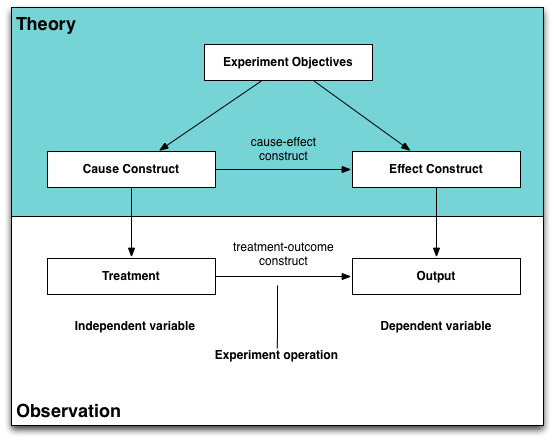
\includegraphics[width=0.5\textwidth]{./images/experiment.png}
\caption{Basic principles behind an experiment}
\label{fig:basic}
\end{figure}

The experiment is created to test a theory or hypothesis. In the design of the experiment, we have a number of treatments over which we have control. The experiment is performed and we are able to observe the outcome. This means that we test the relationship between the treatment and the outcome. If the experiment is properly set up, we should be able to draw conclusions about the relationship between the cause and the effect for which we stated a hypothesis. 

There are two kinds of variables in an experiment, independent and dependent variables. An experiment studies the effect of changing one or more independent variables.
Those variables are called factors. The other independent variables are controlled at a fixed level during the experiment, or else we cannot say if the factor or another variable causes the effect. A treatment is one particular value of a factor

\subsection{Experiment Process}

Figure \ref{fig:experimentprocess} present the experiment process. The starting point for an experiment is insight, and the idea that an experiment would be a possible way of evaluating whatever we are interested in.  Scoping the experiment is the first step. Planning comes next, where the design of the experiment is determined, the instrumentation is considered and the threats to the experiment are evaluated. Operation of the experiment follows from the design. In the operational activity, measurements are collected which then are analyzed and evaluated in analysis and interpretation. Finally, the results are presented and packaged in presentation and package.

\begin{figure}[h]
\center
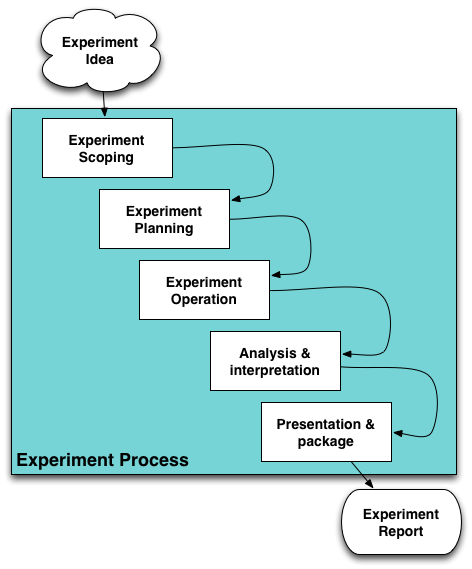
\includegraphics[width=0.4\textwidth]{./images/experimentprocess.png}
\caption{Experiment Process}
\label{fig:experimentprocess}
\end{figure}


The scope of the experiment is set by defining its goals. The planning of the experiment involves the choice of factors, the hypothesis formulation, the selection of variables, the selection of subjects and the the choice of experimentation design \cite{montgomery2008design} \cite{Wohlin2013}.


There are four main types of experiment design \cite{montgomery2008design}:

\begin{itemize}
\item One factor with two treatments. 
\item One factor with more than two treatments. 
\item Two factors with two treatments. 
\item More than two factors each with two treatments.
\end{itemize}


This research aim to compare one factor with two treatments (Record and Playback approach and Search-based approach). In this type of experiment ,we want to compare the two treatments against each other. The most common is to compare the means of the dependent variable for each treatment. The following notations are used:

\begin{itemize}
\item  $\mu_{i}$ The mean of the dependent variable for treatment i .
\item $\gamma_{ij}$ The j:th measure of the dependent variable for treatment i .
\end{itemize}

In this type of experiment is common to use a completely randomized design or a paired comparison design. Randomized design is a basic experiment design for comparing two treatment means. The design setup uses the same objects for both treatments and assigns the subjects randomly to each treatment ( Table \ref{tab:random}).

% Please add the following required packages to your document preamble:
% \usepackage[table,xcdraw]{xcolor}
% If you use beamer only pass "xcolor=table" option, i.e. \documentclass[xcolor=table]{beamer}
\begin{table}[]
\centering
\caption{Example of assigning subjects to the treatments for a randomized design}
\label{tab:random}
\begin{tabular}{|l|l|l|}
\hline
\rowcolor[HTML]{C0C0C0} 
\textbf{Subjects} & \textbf{Treatment 1} & \textbf{Treatment 2} \\ \hline
1                 & X                    &                      \\ \hline
2                 &                      & X                    \\ \hline
3                 &                      & X                    \\ \hline
4                 & X                    &                      \\ \hline
5                 &                      & X                    \\ \hline
6                 & X                    &                      \\ \hline
\end{tabular}
\end{table}

Paired comparison design improve the precision of the experiment by making comparisons within matched pairs of experiment material. In this design, each subject uses both treatments on the same object. This is sometimes referred to as a crossover design. This type of design has some challenges. To minimize the effect of the order, in which the subjects apply the treatments, the order is assigned randomly to each subject. This design cannot be applied in every case of comparison as the subject can gain too much information from the first treatment to perform the experimentwith the second treatment. If we have the same number of subjects starting with the first treatment as with the second, we have a balanced design (Table \ref{tab:paired}).

% Please add the following required packages to your document preamble:
% \usepackage[table,xcdraw]{xcolor}
% If you use beamer only pass "xcolor=table" option, i.e. \documentclass[xcolor=table]{beamer}
\begin{table}[]
\centering
\caption{Example of assigning the treatments for a paired design}
\label{tab:paired}
\begin{tabular}{|l|l|l|}
\hline
\rowcolor[HTML]{FFCCC9} 
\textbf{Subjects} & \textbf{Treatment 1} & \textbf{Treatment 2} \\ \hline
1                 & 2                    & 1                    \\ \hline
2                 & 1                    & 2                    \\ \hline
3                 & 2                    & 1                    \\ \hline
4                 & 2                    & 1                    \\ \hline
5                 & 1                    & 2                    \\ \hline
6                 & 1                    & 2                    \\ \hline
\end{tabular}
\end{table}

In the operation of an experiment a number of parts can be included. Three key parts are \cite{Wohlin2003}:
\begin{itemize}
\item Commit participants: It is important that every participant is committed to the tasks. There are a number of factors to consider, for example, if the experiment
concerns sensitive material, it will be difficult to get committed people.
\item Prepare instrumentation: All the material that should be used during the experiment must be prepared. This may include written instructions to the participants, forms that should be used by the participants during the tests. The instrumentation should be developed according to the design of the experiment. 
\item Execution: The actual execution denotes the part of the experiment where the participants, subject to their treatment, carry out the task that they are assigned to.
For example, it may mean that some participants solve a development assignment with one development tool and the other participants solve the same assignment with another tool. During this task the participants use the prepared instrumentation to receive instructions and to record data that can be used later in analysis.
\end{itemize}

The next step, it is to validate the results. The first part in the actual analysis is normally to apply descriptive statistics. This includes plotting the data in some way to obtain an overview of the data. Part of this analysis is done to identify and handle outliers. After this step, the analysis related to testing one or several hypotheses is performed. Before the results are presented, it is important to assess how valid the results are. The Table \ref{tab:rec} present the tests recommended by each experiment design:

% Please add the following required packages to your document preamble:
% \usepackage[table,xcdraw]{xcolor}
% If you use beamer only pass "xcolor=table" option, i.e. \documentclass[xcolor=table]{beamer}
\begin{table}[]
\centering
\caption{Test recommended by each experiment design}
\label{tab:rec}
\begin{tabular}{|l|l|l|}
\hline
\rowcolor[HTML]{FFCCC9} 
\textbf{Standard Design}                        & \textbf{Param. Tests} & \textbf{N.Param Tests} \\ \hline
One factor with two treatments.                 & t-test                    & Mann-Whitney                  \\ \hline
One factor with two \\ treatments (Paired- Design) & Paired t-test             & Wilcoxon,\\ Sign-test            \\ \hline
One factor with more\\  than two treatments.       & ANOVA                     & Kruskal-Wallis                \\ \hline
Two factors with two treatments.                & ANOVA                     &                               \\ \hline
More than two factors\\ each with two treatments. & ANOVA                     &                               \\ \hline
\end{tabular}
\end{table}



\section{Search-Based Stress Testing}

Search-based testing (SBST) is the process of automatically
generating tests according to a test adequacy criterion using search-based optimization algorithms, which are guided by a fitness function. The role of the fitness function is to capture a test objective that, when achieved, makes a contribution to the desired test adequacy criterion \citep{Harman2010}. 

Search–Based Testing uses metaheuristic algorithms to
automate the generation of test inputs that meet a test
adequacy criterion. An advantage of meta-heuristic algorithms is that they are widely applicable to problems that are infeasible for analytic approaches \citep{Baars2011} \citep{Alba2008}. 

The application of metaheuristic search techniques to test case generation is  a possibility that offers many benefits. Metaheuristic search techniques are high-level frameworks which utilise heuristics in order to find solutions to combinatorial problems at a reasonable computational cost. Such a problem may have been classified as NP-complete or NP-hard, or be a problem for which a polynomial time algorithm is known to exist but is not practical \citep{McMinn2004}.

The search-based stress testing is regarded as a discontinuous, nonlinear, optimization problem, with the input domain of the system under test as a search space \citep{Sullivan}.  The application of SBST algorithms for stress tests involves finding the best- and worst-case execution times (B/WCET) to determine whether timing constraints are fulfilled \citep{Afzal2009a}. 

\subsection{Metaheuristics and Hybrid Metaheuristics}

In the computer science, the term metaheuristic is accepted for general techniques which are not specific to a particular problem. A metaheuristic is formally defined as an iterative generation process which guides a subordinate heuristic by combining intelligently different concepts for exploring and exploiting the search space \citep{raidl2010metaheuristic}. 

Metaheuristics are strategies that guide the search process to efficiently explore the search space in order to find optimal solutions. Metaheuristic algorithms are approximate and usually non-deterministic and sometimes incorporate mechanisms to avoid getting trapped in confined areas of the search space. 

\subsection{Single-Solution Based Metaheuristics}

While solving optimization problems, single-solution based metaheuristics improve a single solution. They could be viewed as "walks" through neighborhoods or search trajectories through the search space of the problem at hand.
 

\subsubsection{Neighborhood}

The definition of Neighborhood is a required common step for the design of any Single-Solution metaheuristic (S-metaheuristic). The neighborhood structure is a important piece in the performance of an S-metaheuristic. If the neighborhood structure is not adequate to the problem,
any S-metaheuristic will fail to solve the problem. The neighborhood function N is a mapping: $ N : S \rightarrow N\textsuperscript{2} $ that assigns to each solution s of \textit{S}, with \textit{N(s)}$\subset$ S \citep{Talbi2013}.

The neighborhood definition depends on the representation associated with the problem. For permutation-based representations, a usual neighborhood is based on the swap operator that consists of swapping the location of two elements $s_i$ and $s_j$ of the permutation \citep{Talbi2013}. The Fig. \ref{fig:sperneighborhood} presents an example where a set of neighbors is found by permutation. 

Single-Solution Based Metaheuristics methods are characterized by a trajectory in the search space. Two common S-metaheuristics methods are Simulated Annealing and Tabu Search.


\subsubsection{Simulated Annealing}

Simulated Annealing (SA) is a randomized algorithm that tries to avoid being trapped in local optimum solution by assigning probabilities to deteriorating moves. The SA procedure is inspired from the annealing process of solids. SA is based on a physical
process in metallurgy discipline or solid matter physics. Annealing is the process of obtaining low energy states of a solid in heat treatment \citep{Jaziri2008}. 

The algorithmic framework of SA is described in Alg. \ref{sa}.  The algorithm starts by generating an initial solution in function \textit{GenerateInitialSolution()}. The initial temperature value is determined in function \textit{SetInitialTemperature()} such that the probability for an uphill move is quite high at the start of the algorithm. At each iteration a solution $\mbox{s}_1$ is randomly chosen in function \textit{PickNeighborAtRandom(N(s))}. If \textit{$\mbox{s}_1$} is better than \textit{s}, then \textit{$\mbox{s}_1$} is accepted as new current solution. Else, if the move from \textit{s} to \textit{$\mbox{s}_1$} is an uphill move, \textit{$\mbox{s}_1$}  is accepted with a probability which is a function of a temperature parameter \textit{Tk} and \textit{s} \citep{raidl2010metaheuristic}. 

\begin{algorithm}[h]
  \caption{Simulated Annealing Algorithm}\label{sa}
  \begin{algorithmic}[1]
    
    \State $s\gets GenerateInitialSolution()$
    \State $k\gets 0 $
    \State $Tk\gets SetInitialTemperature()$
    \While{termination conditions not met }
    \State $\mbox{s}_1\gets PickNeighborAtRandom(N (s))$
    \If{$(f(\mbox{s}_1)<f(s))$}
    \State $s\gets\mbox{s}_1$
    \Else $\;$ Accept $\mbox{s}_1$ as new solution with probability p($\mbox{s}_1|$Tk,s) 
    \EndIf
    \State $K\gets K+1$
    \State $Tk\gets AdaptTemperature()$
    \EndWhile
      
  \end{algorithmic}
\end{algorithm}

\subsubsection{Tabu Search}

Tabu Search (TS) is a metaheuristic that guides a local heuristic search procedure to explore the solution space beyond the local optimal and search with short term memory to avoid cycles. Tabu Search uses a  tabu list to keep track of the last  moves, and prevents retracing \citep{Glover1986}.

The basic idea of TS is the explicit use of search history, both to escape
from the local minima and to implement a strategy for exploring the search space.
A basic TS algorithm uses short term memory in the form of so-called
tabu lists to escape from local minima and to avoid cycles \citep{Tobergte2013}.

The algorithmic framework of Tabu Search is described in Alg. \ref{tsa}.  The algorithm starts by generating an initial solution in function \textit{GenerateInitialSolution()} and the tabu lists are initialized as empty lists in function \textit{InitializeTabuLists($\mbox{TL}_1$,...,$\mbox{TL}_r$)}. For performing a move, the algorithm first determines those solutions from the neighborhood \textit{N(s)} of the current solution \textit{s} that are in the tabu lists. They are excluded from the neighborhood, resulting in a restricted set of neighbors \textit{$\mbox{N}_a(s)$}. At each iteration the best solution \textit{$\mbox{s}_1$} from \textit{$\mbox{N}_a(s)$} is chosen as the new current solution. Furthermore, in procedure \textit{UpdateTabuLists($\mbox{TL}_1$,...,$\mbox{TL}_r$,s,$\mbox{s}_1$)} the corresponding features of this solution are added to the tabu lists.


\begin{algorithm}[h]
  \caption{Tabu Search Algorithm}\label{tsa}
  \begin{algorithmic}[2]
    
    \State $s\gets GenerateInitialSolution()$
    \State InitializeTabuLists($\mbox{TL}_1$,...,$\mbox{TL}_r$)
    \While{termination conditions not met }
    \State $\mbox{N}_a(s)\gets$ $\{\mbox{s}_1 \in N(s) |\mbox{s}_1$ does not violate a tabu condition, or it satisfies at least one aspiration condition $\}$ 
    \State $\mbox{s}_1\gets argmin\{f(\mbox{s}_2)|\mbox{s}_2 \in \mbox{N}_a(s) \}$
    \State UpdateTabuLists($\mbox{TL}_1$,...,$\mbox{TL}_r$,s,$\mbox{s}_1$)
    \State $s\gets \mbox{s}_1$
    \EndWhile
      
  \end{algorithmic}
\end{algorithm}

\subsection{Population-based metaheuristics}

Population-based metaheuristics (P-metaheuristics) could be viewed as an iterative improvement in a population of solutions. First, the population is initialized. Then, a new population of solutions is generated. Finally, this new population is integrated into the current one using some selection procedures. The search process is stopped when a stopping criterion is reached. Algorithms such as Genetic algorithms (GA), scatter search (SS), estimation of distribution algorithms (EDAs), particle swarm optimization (PSO), bee colony (BC), and artificial immune systems (AISs) belong to this class of metaheuristics \citep{talbi2009metaheuristics}. 

\subsection{Genetic Algorithms}

Genetic Algorithms could be a mean of solving complex optimization problems that are often NP Hard. GAs are based on concepts adopted from genetic and evolutionary theories. GAs are comprised of several components \citep{hong2000simultaneously} \citep{shousha2003performance} :

\begin{itemize}
\item a representation of the solution, refered as the chromosome;
\item fitness of each chromosome, refered as objective function;
\item the genetic operations of crossover and mutation which generate new offspring. 
\end{itemize}


Algorithm \ref{gna} shows the basic structure of GA algorithms. In this algorithm, P denotes the population of individuals. A population of offspring is generated by the application of recombination and mutation operators and the individuals for the next population are selected from the union of the old population and the offspring population \citep{raidl2010metaheuristic}.


\begin{algorithm}[h]
  \caption{Genetic Algorithm}\label{gna}
  \begin{algorithmic}[3]
    
    \State $s\gets GenerateInitialSolution()$
    \State Evaluate(P)
    \While{termination conditions not met }
    \State $\mbox{P}_1\gets$ $Recombine(P)$
    \State $\mbox{P}_2\gets$ $Mutate(\mbox{P}_1)$ 
    \State $Evaluate(\mbox{P}_2)$
    \State $P\gets Select(\mbox{P}_2,P)$
    \EndWhile
      
  \end{algorithmic}
\end{algorithm}

\subsection{Hybrid  Metaheuristics}

However, in recent years it has become evident that the concentration on a sole metaheuristic is rather restrictive. A skilled combination of a metaheuristic with other optimization techniques, a so called hybrid metaheuristic, can provide a more efficient behavior
and a higher flexibility when dealing with real-world and large-scale problems \citep{Talbi2012}.

A combination of one metaheuristic with components from other metaheuristics is called a hybrid metaheuristic. The concept of hybrid metaheuristics has been commonly accepted only in recent years, even if the idea of combining different metaheuristic strategies and algorithms dates back to the 1980s. Today, we can observe a generalized common agreement on the advantage of combining components from different search techniques and the tendency of designing hybrid techniques is widespread in the fields of operations research and artificial intelligence \citep{raidl2010metaheuristic}. 

There are two main categories of metaheuristic combinations: collaborative combinations and integrative combinations. Collaborative combinations use an approach where the algorithms exchange information, but are not apart of each other. In this approach, algorithms may be executed sequentially or in parallel. 

One of the most popular ways of metaheuristic hybridization consists of the use of trajectory methods inside population-based methods. Population-based methods are better at identifying promising areas in the search space from which trajectory methods can quickly reach a good local optima. Therefore, metaheuristic hybrids that can effectively combine the strengths of both population-based methods and trajectory methods are often very successful \citep{raidl2010metaheuristic}.


The work uses a type of collaborative combination with sequential execution with two trajectory methods (Tabu Search and Simulated Annealing) and Genetic Algorithms.



\section{IAdapter}

IAdapter is a JMeter plugin designed to perform search-based stress tests.  The plugin is available at \url{www.github.com/naubergois/newiadapter}.  The next subsections present details about the IAdapter Hybrid Approach, the Apache JMeter tool, the IAdapter Life Cycle and the IAdapter Components. The IAdapter plugin provides three main components: WorkLoadThreadGroup, WorkLoadSaver, and WorkLoadController.

\begin{figure}[h]
\centering
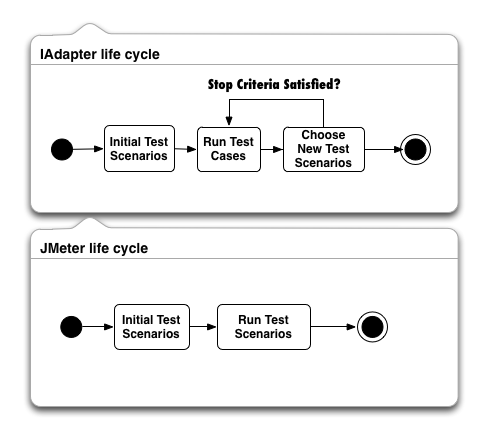
\includegraphics[width=0.5\textwidth]{./images/lifecycle2.png}
\caption{IAdapter life cycle}
\label{fig:iadapterlifecycle}
\end{figure}

The WorkLoadThreadGroup class is the Load Injection and Test Management modules, responsible for generating the initial population and uses the JMeter Engine to send requests to the server under test. 

\subsubsection{IAdapter Life Cycle}
 
Fig. \ref{fig:iadapterlifecycle} presents the IAdapter Life Cycle. The main difference between IAdapter and JMeter tool is that the IAdapter provides an automated test execution where the new test scenarios are choosen by the test tool.  In a test with JMeter, the test scenarios are usually chosen by a test designer.


\subsection{IAdapter Hybrid Approach}

A large number of researchers have recognized the advantages and huge potential of building hybrid metaheuristics. The main motivation for creating hybrid metaheuristics is to exploit the complementary character of different optimization strategies. In fact, choosing an adequate combination of algorithms can be the key to achieving top performance in solving many hard optimization problems \citep{Puchinger2005} \citep{Blum2012}.

The solution proposed by Gois et al. \citep{Gois2016} makes it possible to create a model that evolves during the test. The proposed solution model uses genetic algorithms, tabu search, and simulated annealing in two different approaches. The study initially investigated the use of these three algorithms. Subsequently, the study will focus on other population-based and single point search metaheuristics. The first approach uses the three algorithms independently, and the second approach uses the three algorithms collaboratively (hybrid metaheuristic approach).

In the first approach , the algorithms do not share their best individuals among themselves. Each algorithm evolves in a separate way (Fig. \ref{fig:firstaproach}).





The second approach uses the algorithms in a collaborative mode (hybrid metaheuristic). In this approach, the three algorithms share their best individuals found (Fig. \ref{fig:secondapproach}). The next subsections present details about the used metaheuristic algorithms (Representation, initial population and fitness function).


\begin{figure}[h]
\begin{minipage}{.5\textwidth}
\centering
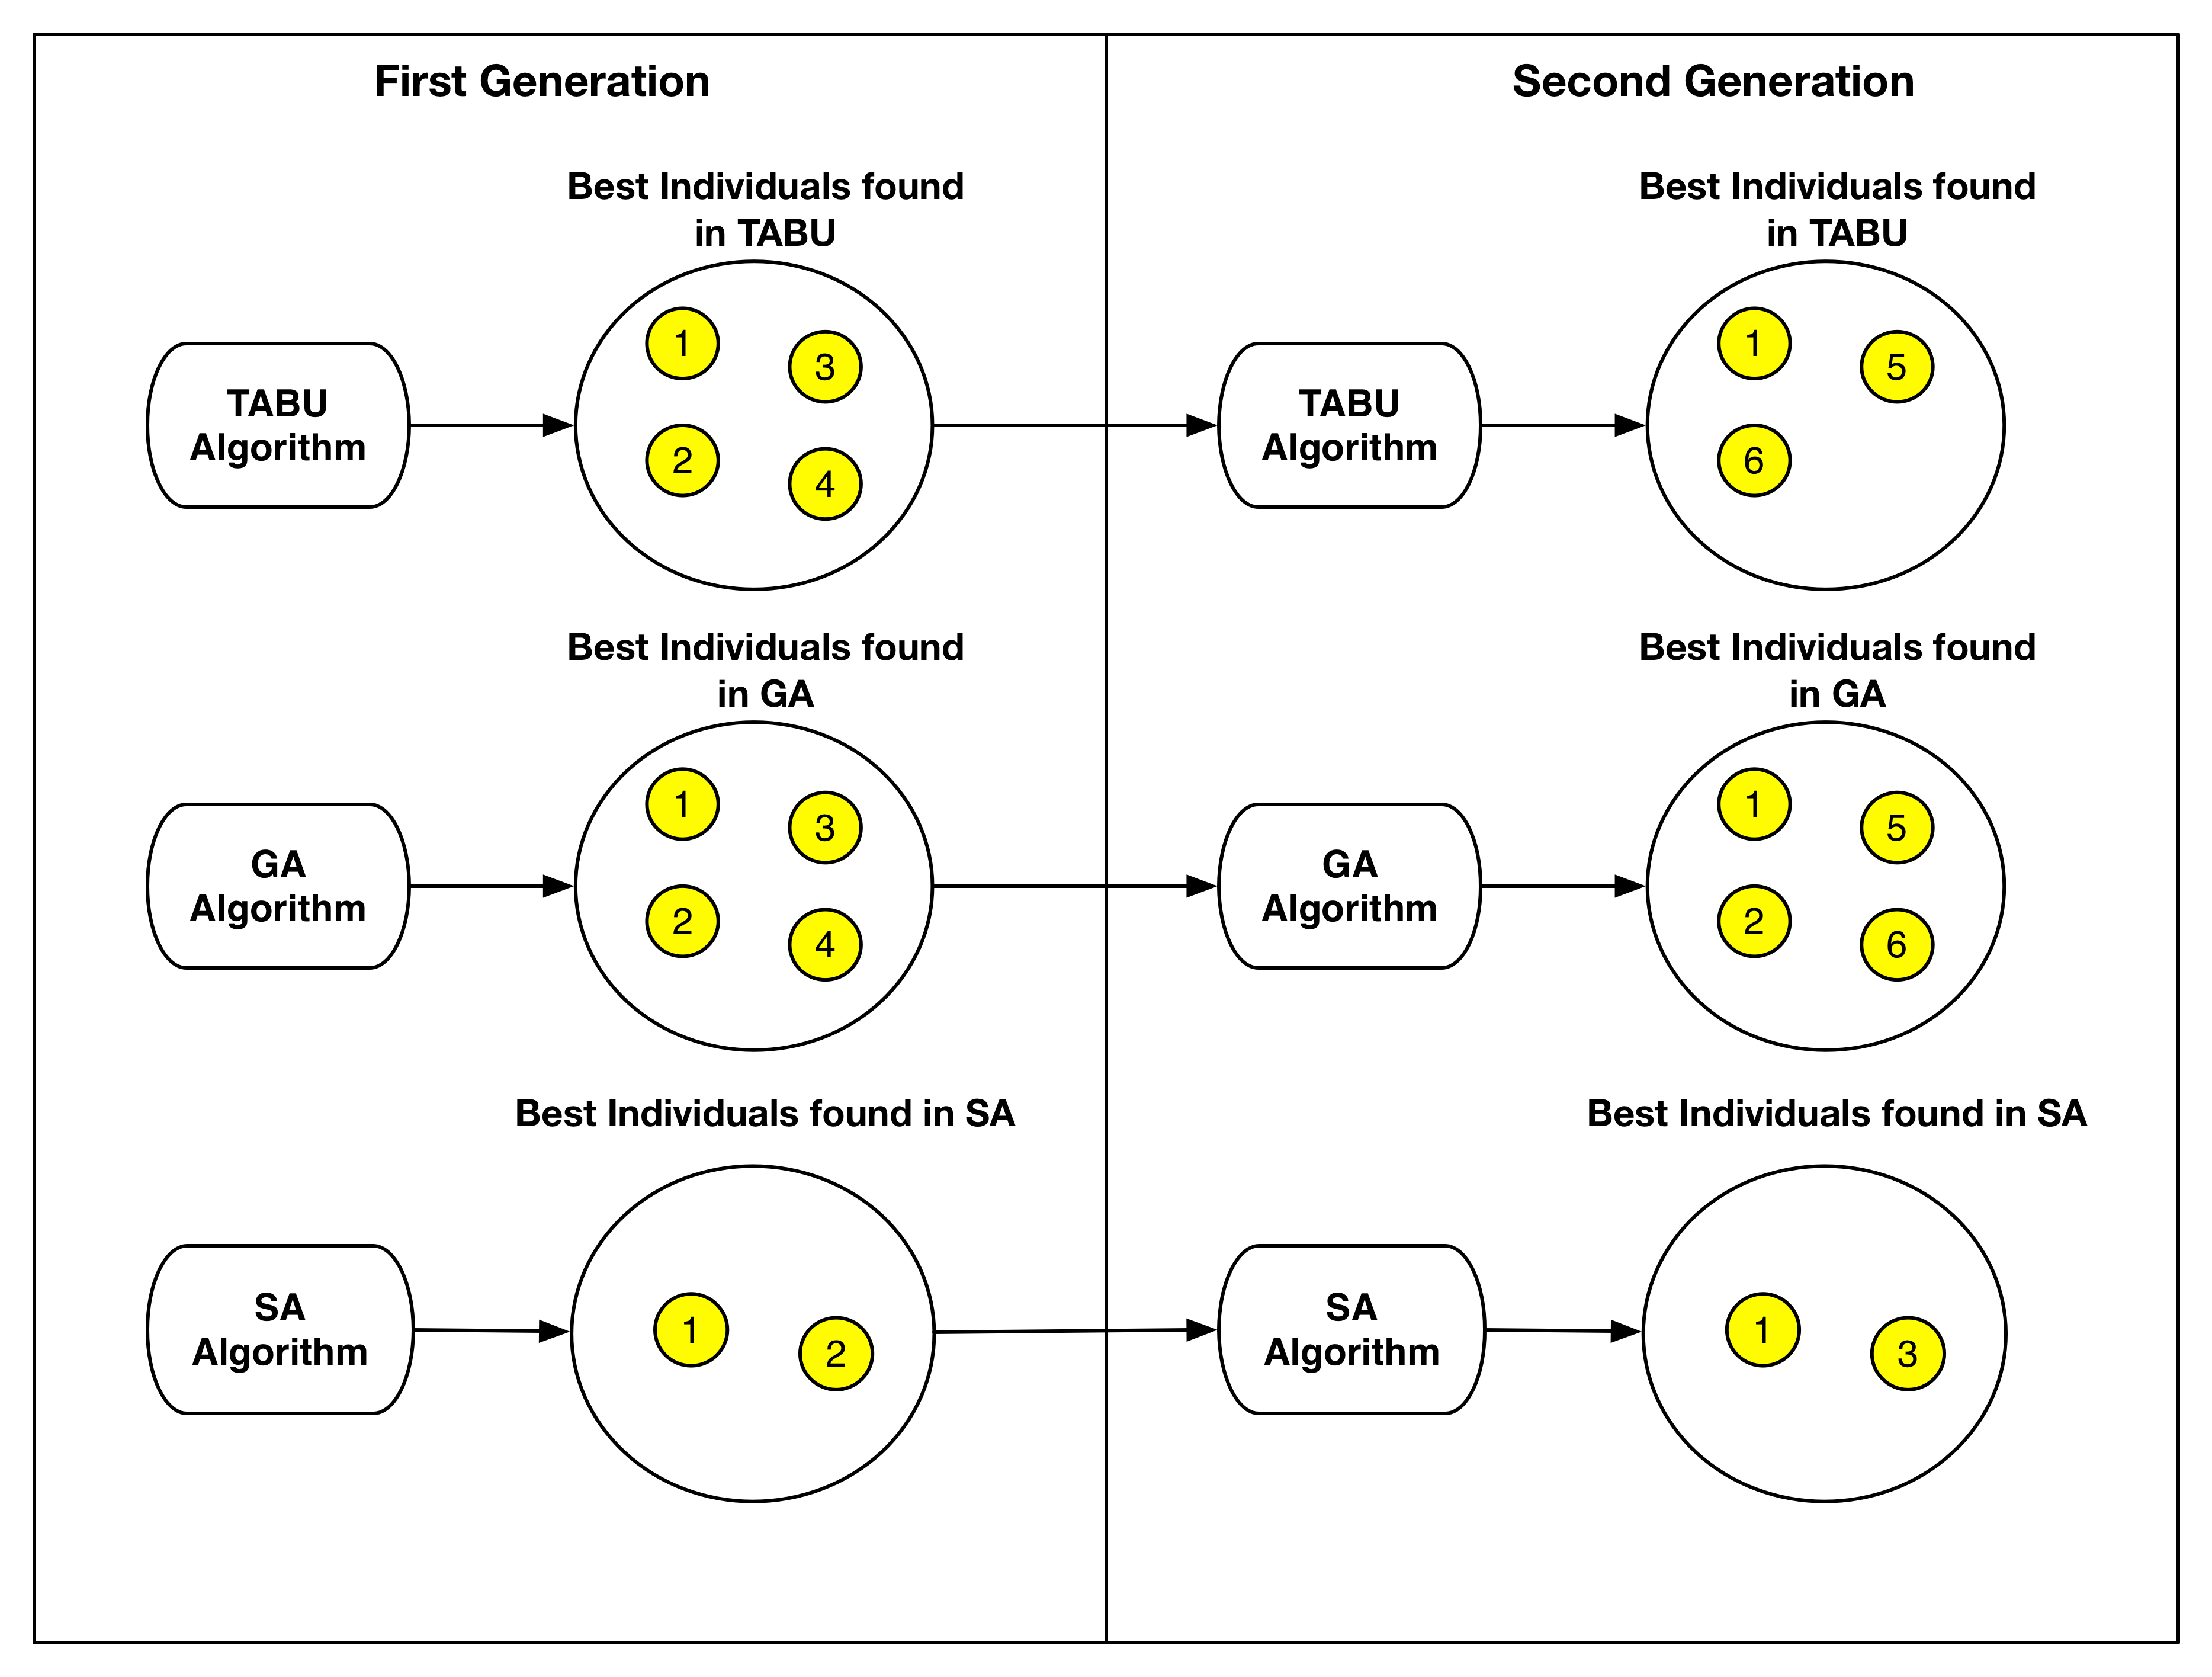
\includegraphics[width=1\textwidth]{./images/independ.png}
\caption{Use of the algorithms independently \citep{Gois2016}}
\label{fig:firstaproach}
\end{minipage}
\begin{minipage}{.5\textwidth}
\centering
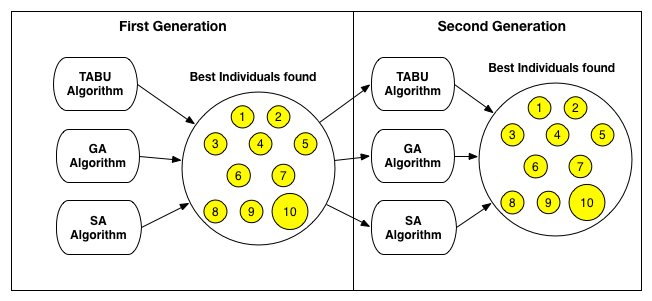
\includegraphics[width=1\textwidth]{./images/collaborative.png}
\caption{Use of the  algorithms collaboratively \citep{Gois2016}}
\label{fig:secondapproach}
\end{minipage}
\end{figure}

\subsubsection{Representation}

The solution representation is composed by a linear vector with 23 positions. The first position represents the name of an individual. The second position represents the algorithm (genetic algorithm, simulated annealing, or Tabu search) used by the individual. The third position represents the type of test (load, stress, or performance). The next positions represent 10 scenarios and their number of users. Each scenario is an atomic operation: the scenario must log into the application, run the task goal, and undo any changes performed, returning the application to its original state.

Fig. \ref{fig:genomarepresentation} presents the solution representation and an example using the crossover operation. In the example, genotype 1 has the Login scenario with 2 users, the Form scenario with 0 users, and the Search scenario with 3 users. Genotype 2 has the Delete scenario with 10 users, the Search scenario with 0 users, and the Include scenario with 5 users. After the crossover operation, we obtain a genotype with the Login scenario with 2 users, the Search scenario with 0 users, and the Include scenario with 5 users.

\begin{figure}[h]
\begin{minipage}{.5\textwidth}
\centering
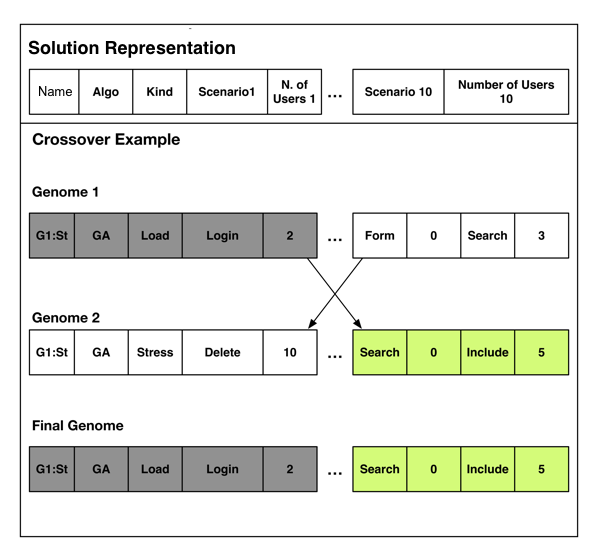
\includegraphics[width=1\textwidth]{./images/genomerepresentation1.png}
\caption{Solution representation and crossover example \citep{Gois2016}}
\label{fig:genomarepresentation}
\end{minipage}
\begin{minipage}{.5\textwidth}
\centering
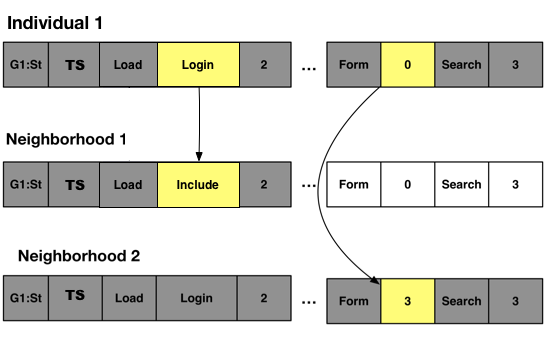
\includegraphics[width=1\textwidth]{./images/neighbor.png}
\caption{Tabu search and simulated annealing neighbor strategy \citep{Gois2016}}
\label{fig:neighbourtaby}
\end{minipage}
\end{figure}

Fig. \ref{fig:neighbourtaby} shows the strategy used by the proposed solution to obtain the representation of the neighbors for the Tabu search and simulated annealing algorithms. The neighbors are obtained by the modification of a single position (scenario or number of users) in the vector.

\subsubsection{IAdapter Components}
 
WorkLoadThreadGroup is a component that creates an initial population and configures the algorithms used in IAdapter. Fig. \ref{fig:tela1iadapter} presents the main screen of the WorkLoadThreadGroup component. The component has a name \ding{202}, a set of configuration tabs \ding{203}, a list of individuals by generation \ding{204}, a button to generate an initial population \ding{205}, and a button to export the results \ding{206}.

\begin{figure}[h]
\centering
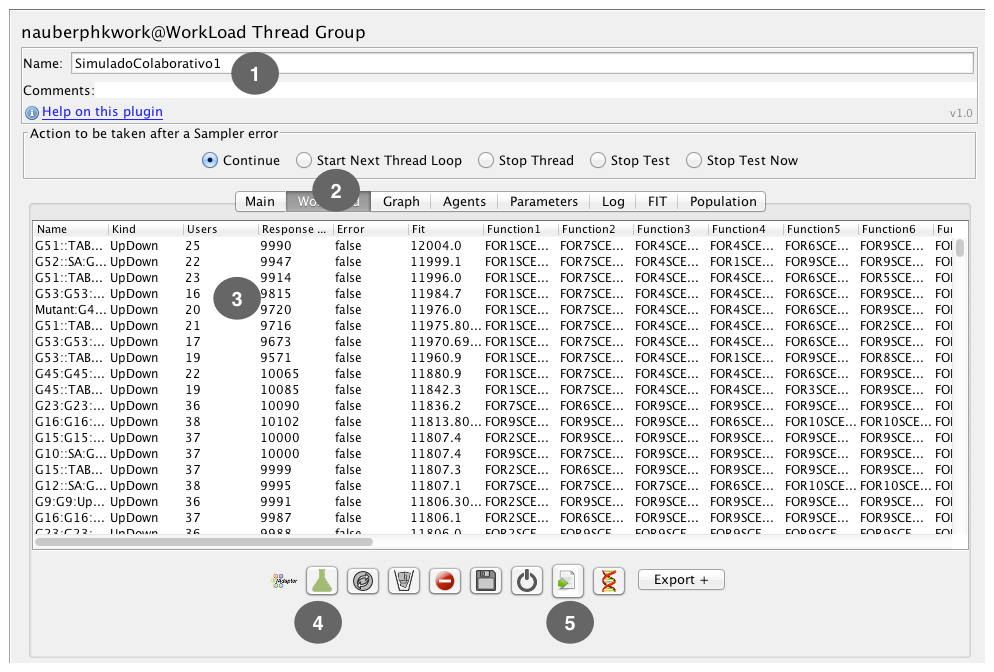
\includegraphics[width=0.5\textwidth]{./images/tela1iadapter.png}
\caption{WorkLoadThreadGroup component}
\label{fig:tela1iadapter}
\end{figure}

WorkLoadThreadGroup component uses the GeneticAlgorithm, TabuSearch and SimulateAnnealing classes.  The WorkLoadSaver component is responsible for saving all data in the database. The operation of the component only requires its inclusion in the test script.

WorkLoadController represents a scenario of the test. All actions necessary to test an application should be included in this component. All instances of the component need to login into the application under test and bring the application back to its original state.

\section{Experiment}

\subsection{Scope of experiment}

The scope of of the experiments is analyze the application of stress search-based test for the purpose of evaluation with respect to effectiveness and efficienct from the point of view of the test designer in the context of an stress test industrial practices.  

\subsection{Research Questions}

The following research question is addressed:
\begin{itemize}
\item Does the approach used by IAdapter manage to find scenarios with a larger number of users within the established maximum response time?
\end{itemize}

The experiment consist on execute a test script in two different situations:

\begin{itemize}
\item The first situation consist on execute the script using the Apache JMeter 2.3  configured according with the parameters choosen by each test designer.
\item The second situation consist on execute the script with the IAdapter JMeter plugin.
\end{itemize}

\subsection{Variables}

The independent variables are the test approach (JMeter apprach or IAdapter approach). The dependent variable are the number of users  within the established maximum response time.

\subsection{Hypotheses}

\begin{itemize}

\item With regard to the maximum number of users found in the experiment:

\begin{itemize}
\item $H_{0}$ (A null hypothesis) : the number of users found with the iadapter plugin is minor or equal to use the default jmeter configuration.
\item $H_{1}$  : the number of users found with the iadapter plugin is major than the default jmeter configuration.
\end{itemize}


\end{itemize}


\subsection{Selection of Subjects}

The subjects are chosen based on convenience, i.e. the subjects are test designers assigned to the federal data-processing service, a state-run Brazilian federal government.


\subsection{Experiment design}

The experiment use a paired comparison design. 

\subsection{Experiment validation}

The experiment results was validated with Paired t-test.

\section{Survey}

\subsection{Research Questions}

The following two questions are addressed:
\begin{itemize}
\item Is using combined test scenarios a necessity in stress testing?
\item Is the IAdapter tool easier to use than Apache JMeter?
\end{itemize}

\subsection{Hypotheses}

The survey have two hypotheses:

\begin{itemize}

\item Concerning the need to test combined test scenarios in stress tests

\begin{itemize}
\item $H_{0}$ (A null hypothesis) : It is not necessary to test combined scenarios on stress tests.
\item $H_{1}$  : It is  necessary to test combined scenarios on stress tests.
\end{itemize}


\item Regarding the ease of use of each tool: 


\begin{itemize}
\item $H_{0}$ (A null hypothesis) : The Apache JMeter tool was easier to use than the IAdapter plugin.
\item $H_{1}$  : The IAdapter plugin tool was easier to use than the default Apache JMeter.
\end{itemize}

\end{itemize}




\bibliographystyle{ACM-Reference-Format}
\bibliography{sigproc} 

\end{document}
